
\chapter{Findings}\label{chapter:findings}
This chapter will discuss our findings on bugs related to accelerators and \ac{TCG}.
We will begin by examining the distribution of bugs in \ac{QEMU} to understand the impact of accelerator bugs on development.
Then, we will discuss bugs caused by accelerators, followed by a list of bugs found in different accelerator target architectures.
Special attention will be given to x86 architectures as targets.
Additionally, we will delve into bugs that specifically occur on Arm CPUs when running x86 binaries in order to explore whether \ac{QEMU} has additional bugs depending on the host architecture.

Before we start, it is essential to note that this survey is based on data from \ac{QEMU}'s GitLab repository \cite{qemu_issues}.
As of this writing, there are 2140 issues, with the oldest dating back to 2021.
Some bugs have been transferred from the previous repository, making it challenging to determine their exact date.
Figure \ref{fig:issues} shows the distribution of relevant bugs for reference.

\begin{figure}[ht]
    \centering
    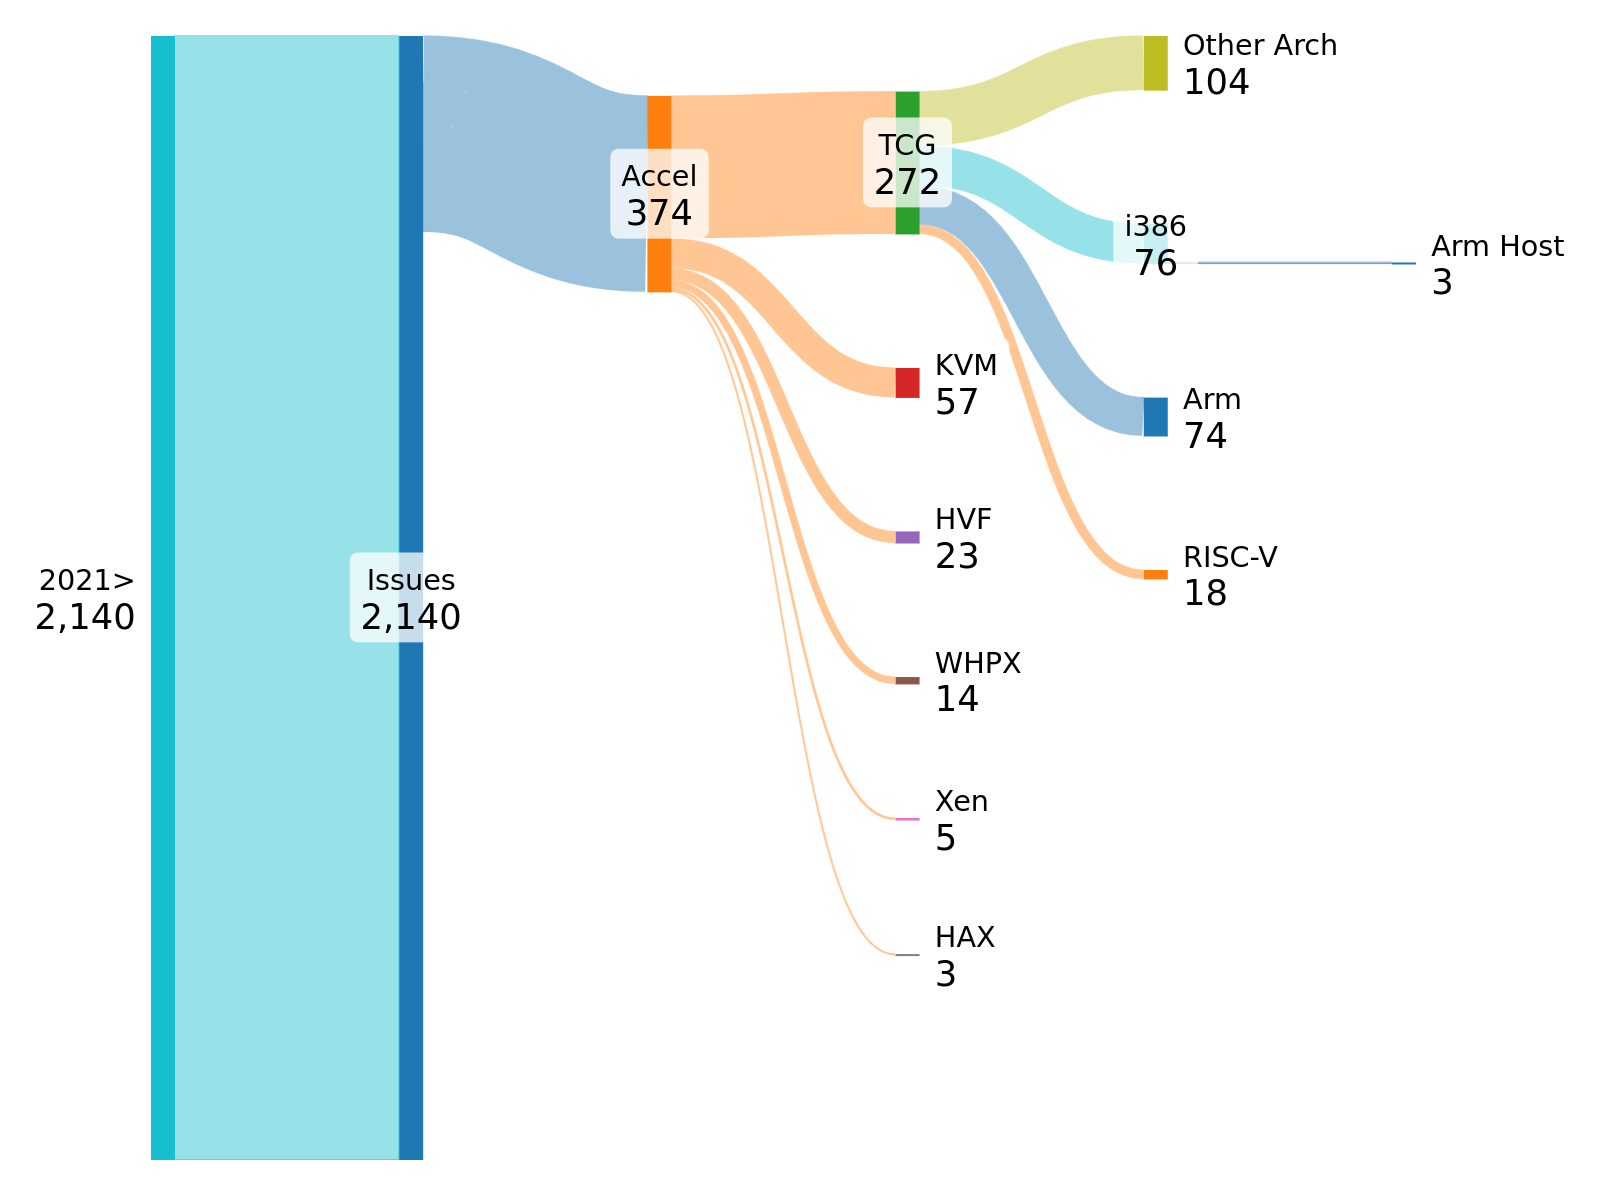
\includegraphics[width=0.8\linewidth]{figures/issues3}
    \caption[QEMU bug distribution]{Sankey diagram showing the distribution of relevant issues}
    \label{fig:issues}
\end{figure}

\section{Distribution of Bugs in \ac{QEMU}}
As shown in figure \ref{fig:issues}, \ac{QEMU} currently has over 2000 bugs.
According to the line counting program cloc \cite{cloc}, the newest version of \ac{QEMU} has 2038147 \ac{sloc} split between different programming and scripting languages.
Drawing from Steve McConnell's research on software metrics \cite{sloc}, we can compare \ac{QEMU}'s bug frequency to that of commercially released products, indicating that \ac{QEMU} has a relatively clean codebase.

There are 374 bugs related to accelerators, accounting for about 15\% of the total.
This percentage suggests that the accelerator-related issues are a significant part of the total bugs.
Among these accelerator bugs, the majority, or about 70\%, stem from \ac{TCG}, which is expected given that \ac{TCG} is the primary and most widely used accelerator.
KVM-related bugs make up another 15\%, with the remaining 15\% spread across other accelerators.

Regarding \ac{TCG} specific bugs, those involving x86 (i386) and Arm architectures are the most common, each being roughly around 30\% of the total.
This should not be surprising since these architectures are most commonly utilized, leading to extensive usage and, therefore, testing.

\section{x86 Translation Errors}
This section will review the bugs encountered when running x86 binaries using the \ac{TCG}.
Most of these bugs are independent of host architecture and operating system and tend to arise from incorrect implementation of individual instructions.

We have organized these bugs into six categories based on how they affect the emulation:
\begin{itemize}
    \item Calculation Error: These are mistakes in instructions that either lead to incorrect calculations or issues with flag registers being incorrectly set or not set at all. However, they do not usually interrupt the flow of the program. They happen because of wrong instruction implementation.
    \item Exceptions: These bugs trigger an exception in \ac{QEMU}, causing the emulation to stop abruptly.
    \item Errors: Similar to exceptions, these issues cause \ac{QEMU} to halt the emulation process.
    \item Segmentation Faults: These occur when the program attempts to access memory areas it does not have permission to access. While this does not happen on actual hardware, it is triggered during the emulation.
    \item Hardware Problems: These bugs impact external hardware, potentially making it unusable or inefficient.
    \item Other Bugs: This category includes bugs that do not fit into the other groups because their origin is unclear or because they were introduced in newer versions by mistake.
\end{itemize}

The results of the survey are expressed in the table \ref{tab:tcg_x86}.
The following sections will mainly focus on calculation errors since the verifier excels at this area.
Testing other bugs would be challenging since they do not necessarily finish their execution normally, leaving the emulator logs incomplete.
This topic will be discussed in chapter \ref{chapter:future_work}.

\begin{table}[htpb]
    \caption[x86 TCG error distribution]{Distribution of TCG errors for x86.}\label{tab:tcg_x86}
    \centering
    \begin{tabular}{l r r r}
      \toprule
        Type & Number & Closed & Open \\
      \midrule
        Calculation Error & 18 & 12 & 6 \\
        Exceptions & 6 & 4 & 2 \\
        Errors & 3 & 2 & 1 \\
        Segmentation Faults & 14 & 10 & 4 \\
        Hardware Problems & 1 & 0 & 1 \\
        Other & 33 & 26 & 7 \\
      \bottomrule
    \end{tabular}
\end{table}

\subsection{Interpretation and Evaluation of the Bug Survey}

\paragraph{Other:}
As shown in table \ref{tab:tcg_x86}, most errors originating from x86 emulation belong to this category.
Moreover, these errors make up nearly 45\% of the total amount.
Unfortunately, the bugs that cause these problems are multiple and complex; therefore, they cannot be easily traced to simple instructions.
A good example of these types of bugs would be bug \#661 \cite{qemu_661}, which only appeared after version 6.1 of \ac{QEMU}.
This bug would cause \ac{QEMU} to freeze after enabling 5 level paging, and it was traced to missing bit masks that prevented consistency checks for CR4.
In this case the verifier should be able to trace the bug to a move instruction which enables 5 level paging.
However, since \ac{QEMU} freezes without transitioning to the next state, the emulator log would be insufficient, and the verifier cannot detect it.

Depending on the complexity, the verifier can find the bug, and the reproducer might be able to reproduce it.
However, it is more than likely that the steps that result in these bugs cannot be repeated to pinpoint the actual reason.
Therefore, it is difficult to reproduce them, making our project a lousy match against them.

\paragraph{Hardware Problems:}
These kinds of bugs are likely to result from problems in IO.
Therefore, they are out of this project's scope since we are explicitly interested in translation errors.


\paragraph{Segmentation Faults:}
These bugs are another frequent issue, accounting for nearly 20\% of all bugs.
A \ac{segfault} happens when a program attempts to access a nonexistent or restricted area.
These accesses can be classified into three categories:
\begin{itemize}
  \item Read
  \item Write
  \item Execute
\end{itemize}
Generally, the best way to solve these bugs is to trace them and find where they caused the \ac{segfault}.
In most cases an emulator will keep running and outputting the emulator log until one of the aforementioned events happens.
After the \ac{segfault} happens, the program will be stopped abruptly, and the emulator will stop.
This means the emulator log will be stopped before reaching the end.
Even though the emulator trace will be cut off in the case of a segmentation fault, considering that we only need to find the address where this happens along with the used instructions, the verifier can be helpful.

Although the verifier can prepare the snapshot and the symbolic expression, the current version only finds errors by comparing states.
This means it will stop before noticing that the emulator log is short.
Theoretically, if the \ac{segfault} is happening because of an instruction, the reproducer should be able to reproduce it. 
However, in most cases, this is not possible since the reproducer ignores some details.
A \ac{segfault} happens for multiple reasons, either because the memory location does not have the required permissions or does not exist.
However, neither the verifier nor its symbolic log has any knowledge about a memory location's permissions.
Therefore, even if we can extract the offending instruction and the used values without being able to set the memory location's permissions, we cannot set an equivalent environment.

In this case, we have two choices.
We can handle it like other memory access instructions, allocating space on the data section and then using it for reading or writing.
Alternatively, we can keep the original address.
In the first case, we will likely avoid triggering the fault since we use the location we declared and ensured it exists.
In the second case, we have yet to determine whether this original address exists and its value and permissions.
Therefore, this method would cause undefined behavior.
Because of these reasons, the reproducer is not a good match for this type of error.
The best we can expect to do is to try the first way and see whether we can trigger the \ac{segfault} consistently.

\paragraph{Errors and Exceptions:}
Errors and exceptions are relatively common in \ac{QEMU}, leading to the program stopping. These issues likely stem from the emulator's internal state, suggesting that alternative debugging methods might be more effective.

\paragraph{Calculation Errors:}
Finally, we have the calculation errors.
They make up slightly less than 25\% of total errors, but they are theoretically the most challenging to detect as they involve instructions behaving slightly differently than expected.
For example, some instructions might set a bit to a wrong value or change another bit that it should not touch.

The main problem with these instructions is that these values are not necessarily used.
They may stay hidden since they might not be used or overwritten by different instructions.
This means these programs can go a long way before exhibiting the bug since the difference might have happened multiple instructions ago.
Alternatively, the result may be close enough to the expected answer so the bug might not be detected.

However, in a good case, this instruction calculates wrong values, and this discrepancy is detected.
Our verifier and reproducer combination matches these instructions well since it uses symbolic execution to model every state transformation and compare it with the emulator log.

\subsection{Detailed Inspection of Bugs on Arm}
In the following subsections, we will review specific bugs that only appear on Arm devices.
We thoroughly inspect these bugs because we want to see whether some bugs appear depending on the host hardware.
Out of 76 bugs we have seen, only 3 are Arm-specific.
Considering this fact, we can assume that hardware-specific bugs are relatively rare.
After examining the following subsections, it should be clear that these bugs are not caused by the host architecture but by other factors.

\subsubsection{Issue \#1659 \cite{qemu_1659}}
The first issue specific to Arm was discovered in an aarch64 system running Darwin.
This bug caused the emulator to freeze and enter a continuous shutdown loop.
It was traced back to the floatx80\_div instruction.
Upon closer examination, it was determined that the problem was due to a miscompilation by Clang.

Therefore, this issue is not directly related to the emulator but to the compiler, meaning we can cross it off the Arm-only list.

\subsubsection{Issue \#2101 \cite{qemu_2101}}
The second issue was identified on a system using Fedora Linux as the host.
This bug manifests when executing the ls command within \ac{QEMU}.
It results in incorrect output that omits several directories.
Due to the lack of more information, it is not possible to find the actual cause.

\subsubsection{Issue \#2168 \cite{qemu_2168}}
The final issue also happens in Linux.
This time, a segmentation fault occurs when running grep on Gentoo Linux inside \ac{QEMU}.
Similar to the previous issue, limited information is available, making it difficult to provide more insights.
